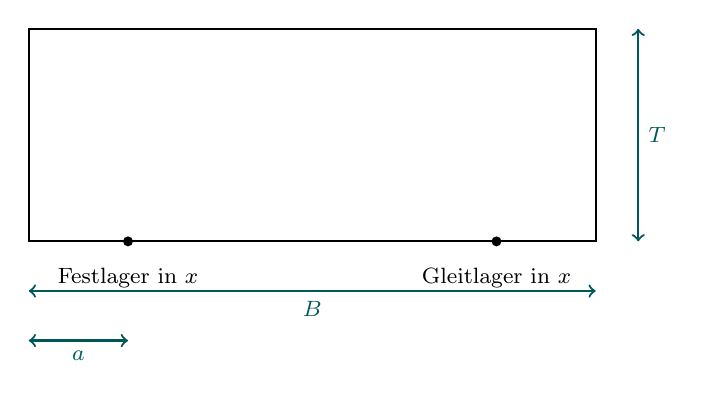
\begin{tikzpicture}[scale=0.9, every node/.style={font=\footnotesize}]
\draw[thick] (0,0) rectangle (8,3);
\fill (1.4,0) circle (2pt) node[below=6pt]{Festlager in $x$};
\fill (6.6,0) circle (2pt) node[below=6pt]{Gleitlager in $x$};
\draw[<->,teal!70!black,thick] (0,-0.7)--(8,-0.7) node[midway,below]{$B$};
\draw[<->,teal!70!black,thick] (8.6,0)--(8.6,3) node[midway,right]{$T$};
\draw[<->,teal!70!black,thick] (0,-1.4)--(1.4,-1.4) node[midway,below]{$a$};
\end{tikzpicture}
